\documentclass[../Main.tex]{subfiles}

\begin{document}
\section*{\crule[blue]{.3cm}{.3cm} Introduction}
Phytoplankton blooms are sudden explosive increases in phytoplankton. They occur when nutrient and sunlight conditions are just right and can last several weeks. The timing of these blooms plays a large role in maintaining marine ecosystems and is crucial to the survival of certain fish and bird species. However, there are also harmful phytoplankton blooms bringing death or disease killing marine life, because certain species of phytoplankton produce powerful biotoxins. \supercite{Prim2021}

Phytoplankton are microscopic organisms living in watery environments, both salty and fresh. Most are single-celled plants, some are bacteria and some protists. The life span of any individual phytoplankton is rarely more than a few days. \supercite{Prim2021}

Phytoplankton plants are primary producers and are starting the aquatic food web. They typically float close to the surface, where there is sunlight for photosynthesis and is feeding everything from microscopic zooplankton, small fish and invertebrates to huge whales. In the marine food chain smaller animals are then eaten by bigger ones etc. \supercite{Prim2021}

To understand the initiation of phytoplankton blooms depending on the amount of nutrients and sunlight the concepts critical depth and compensation depth are useful. Compensation depth is the depth where the rate of organic matter by photosynthesis is equivalent to the rate of decomposition of organic matter by plant respiration. The critical depth is the depth where solar radiation can just balance radiation.\supercite{Sverdrup1953OnCF}




\begin{figure}[H]
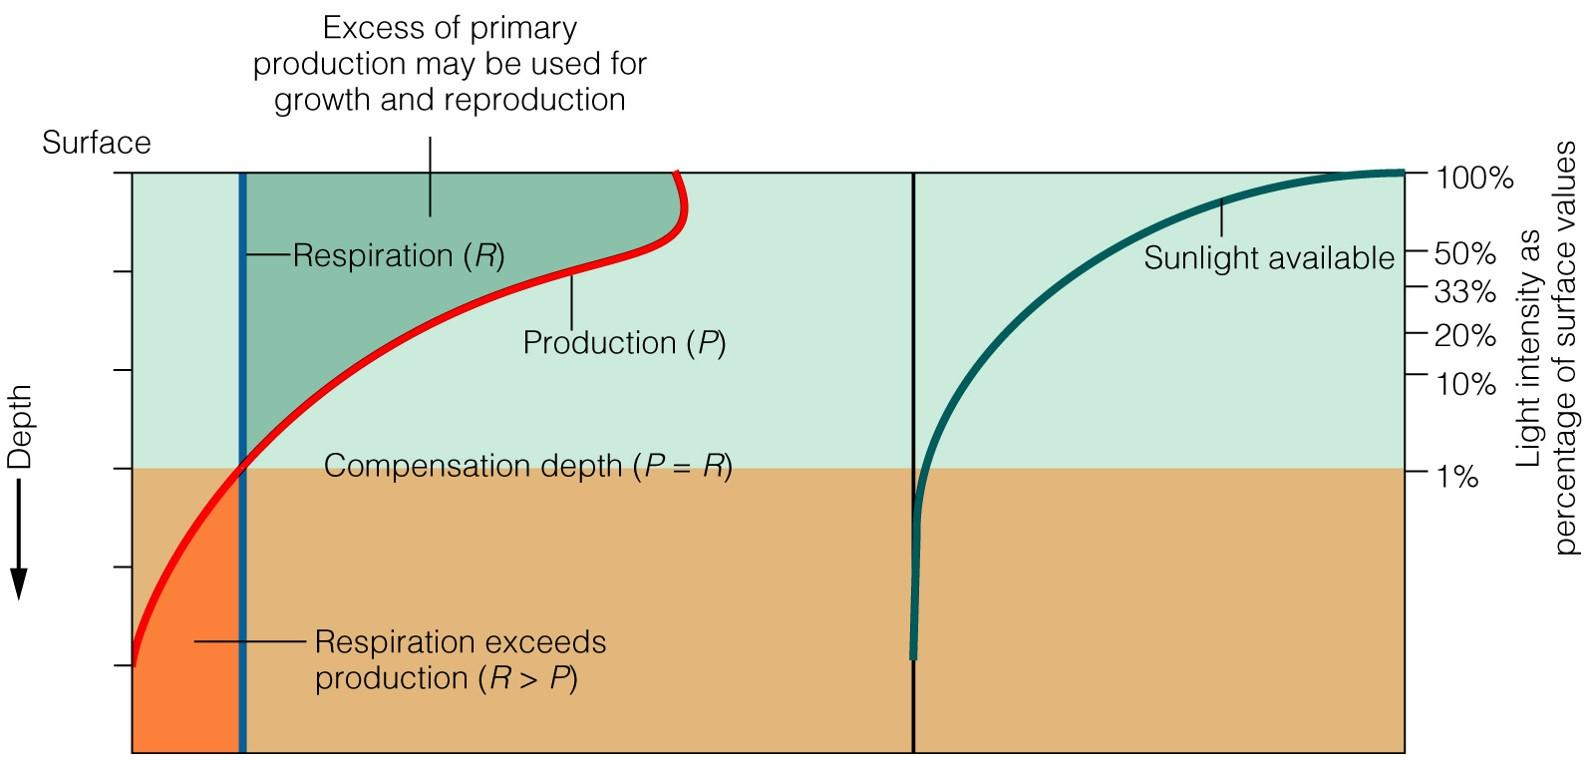
\includegraphics[width=8cm]{Primary_Production.jpg}
\caption{The relationship between the water depth and net primary production (=P-R) \supercite{Nasa2021}}
\end{figure}
Phytoplankton blooms can be studied in many ways such as by scientists on research vessels taking samples and monitoring onboard with technical equipment, long term moored boys, satellite instruments and unmanned underwater vehicles including remotely operated underwater vehicles (ROVs) and autonomous underwater vehicle (AUV).  

Autonomous underwater vehicles have recently become an attractive alternative for underwater search and exploration since they are cheaper than manned vehicles.  An autonomous underwater vehicle (AUV) is a robot travelling underwater without requiring input from an operator. 

Gliders are one type of autonomous underwater vehicles able to remain at sea for long periods of time while continuously collecting data from a range of disciplines at high resolution. It has its advantages with lower costs and accuracy compared to other ways of collecting data, but there are also from time-to-time difficulties with the equipment and controlling it The equipment and work methods are still on quite an early stage of development. There are also other factors affecting and restricting the use of them such as shipping and fishing. Besides state and international permits are needed to use them, which can be difficult to get. 

Gliders were used in collecting data for this study, which is analysing the evolution of phytoplankton through blooms in the Bornholm basin. The data was collected within the infrastructure project Smart Autonomous Monitoring of the Baltic Sea (SAMBA) funded by the Voice of the Ocean Foundation. 
The mission and purpose of the Voice of the Ocean Foundation, run by a group of oceanographers, historians and entrepreneurs, is to “conduct, support and promote science, education, information and communication regarding the sea, marine ecosystems, and the marine environment as well as the interaction between man and the sea, historically, at the present time and in the future.”\supercite{VOTO2021}
VOTO - Voice of the Ocean Foundation
https://voiceoftheocean.org

The observations are run by a group of oceanographers, technicians and a piloting team since March 2021 on two locations, Skagerrak and in the Bornholm basin. The project is combining short term science objectives and the long-term vision of establishing several persistent ocean observatories across the Baltic Sea for international collaboration. 

The focus of this report is the Bornholm basin located in southwest of the Baltic Sea. We have been studying and analysing the continuous gliders data since March 2021 from French built “Sea Explorer” sea gliders. They are collecting data such as ADCP backscatter, PAR (light), salinity, temperature, positions, chlorophyll a, and turbidity with the aim to describe potential physical drivers behind the productivity such as for example mixed layer depth dynamics, light availability and euphotic depth, wind stress and heat fluxes. 
\begin{figure}[H]
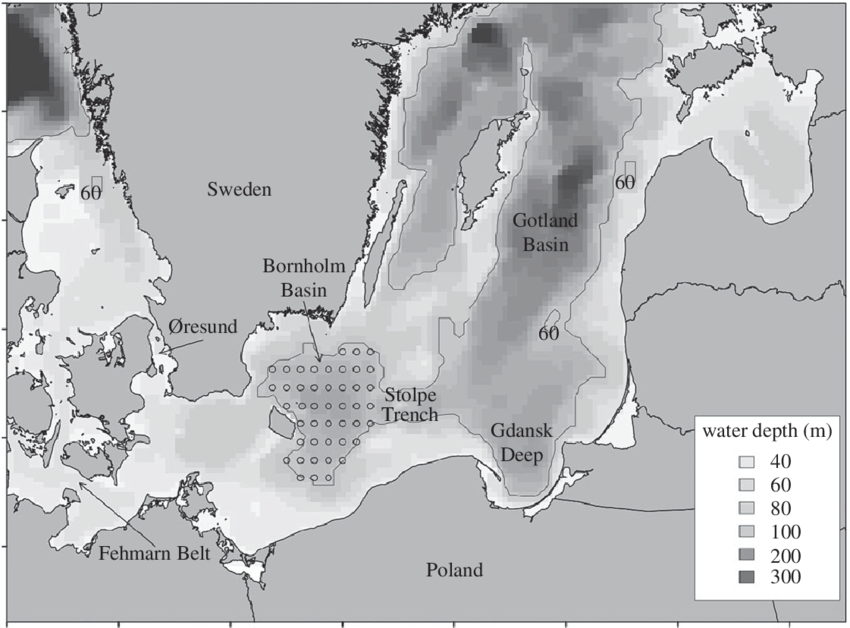
\includegraphics[width=8cm]{Location.jpg}
\caption{The location of the Bornholm Basin}
\end{figure}
This study is evaluating some of these data, giving insight into two phytoplankton blooms occurring from during the period March to October 2021, as a project part of the course MAR440 Marine Project from idea to realization at University of Gothenburg the autumn 2021.


\end{document}
